\chapter{Lecture 4 - Newton's Method and Secant Method}
\label{ch:lec4n}
\section{Objectives}
The objectives of this lecture are to:
\begin{itemize}
\item Describe and demonstrate Newton's method for solving non-linear equations.
\item Illustrate the convergence properties of Newton's method and highlight convergence issues.
\item Introduce and demonstrate the secant method.
\end{itemize}
\setcounter{lstannotation}{0}

\section{Introduction}
Bracketing methods described in the previous note had at least two issues:
\begin{enumerate}
\item End-points for the bracket $\left[a,b\right]$ in which a root is contained needed to be determined.  There is no cut-and-dried sure-fire way to accomplish this task.  Luckily, a suitable bracket can often be found even if such a method is hard to automate and may feel a bit ``cluncky.''

\item The convergence rate is ``slow''---although we have not yet described any competing methods that are ``faster'' such that a proper perspective can be gained.
\end{enumerate}
The open methods to be described in this lecture eliminate the first drawback of bracketing methods; open methods need no bracket containing a root, only an initial starting point.  Also, it will be shown, that the open methods described in this note converge more quickly than bracketing methods such as the bisection algorithm thereby clarifying the impact of the second drawback. 

On the other hand, these open methods will introduce additional complications that offset some of their advantages.  these issues will be described and options for mitigating these complications will be presented.

\section{Newton's Method}

\begin{marginfigure}
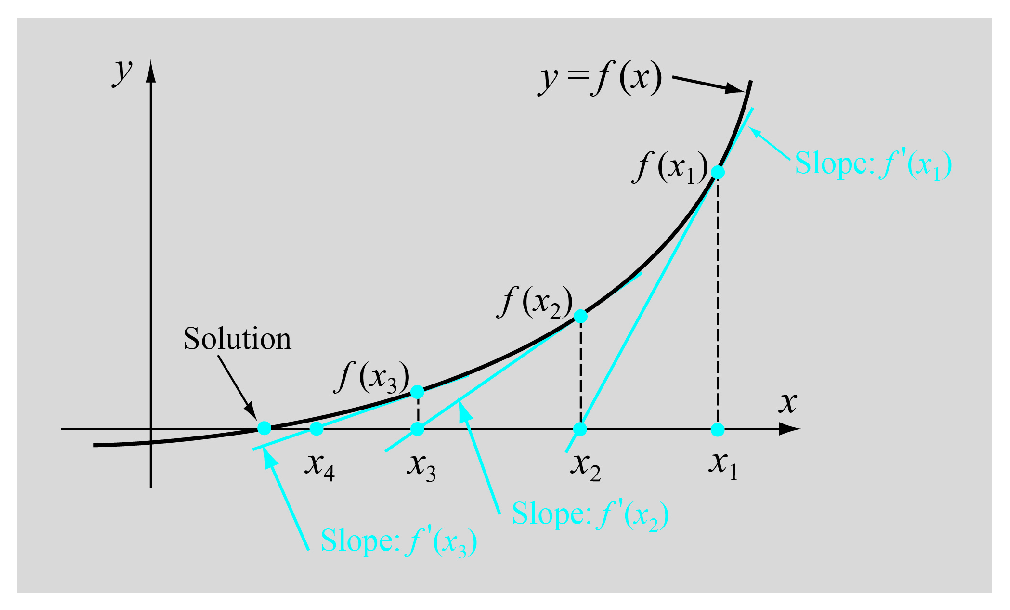
\includegraphics{Chapter3_Fig3_10.eps}
\caption{The first four iterations of Newton's method.}
\label{fig:newton-schematic}
\end{marginfigure}
Newton's method, also called the Newton-Raphson method, is a classic method for finding roots of equations that are \emph{continuous} and \emph{differentiable}. Given an initial estimate of the solution $x_1$, the second estimate is determined by taking the tangent line to $f(x)$ at the point $[x_1,f(x_1)]$ and finding the intersection of the point of the tangent line with the $x$-axis. A schematic of the first four iterations of Newton's method is shown in Figure \ref{fig:newton-schematic}.  Successive estimates are found in the same way.  The slope of the tangent line at $x_1$ is denoted $f^{\prime}(x_1)$.  The point $x_2$ is determined from Equation \ref{eq:lec4n-newton-update}.\marginnote{\textbf{Note:} The expression for $x_2$ given in Equation \ref{eq:lec4n-newton-update} is obtained from: 

$$ f^{\prime}(x_1) = \frac{f(x_1)-0}{x_1 - x_2}$$
}
\begin{equation}
x_2 = x_1 - \frac{f(x_1)}{f^{\prime}(x_1)}
\label{eq:lec4n-newton-update}
\end{equation}
This process can ge generalized for finding solutions $x_{i+1}$ from $x_i$ as shown in Equation \ref{eq:lec4n-newton-update2}.
\begin{equation}
x_{i+1} = x_{i} - \frac{f(x_i)}{f^{\prime}(x_i)}
\label{eq:lec4n-newton-update2}
\end{equation}
The algorithm for Newton's method can be states as follows:
\begin{enumerate}
\item Choose a point $x_1$ as an initial guess of the solution.
\item For $i = 1,2,\dots,$ until the error is smaller than a specified tolerance, use Equation \ref{eq:lec4n-newton-update2} to find $x_{i+1}$ and repeat.
\end{enumerate}


\newthought{Since this is not} a bracketing method, we do not have a ``bracket'' to use in estimating the solution error like we did in the bisection or regula falsi method.  There are a couple of stopping criteria that could be used:
\begin{enumerate}
\item Tolerance in $f(x)$.  Recall from the last lecture, this means we will stop the iteration when, for some specified tolerance $\delta$, the following relation is satisfied:
\begin{equation}
\left| f(x_i) \right| \le \delta
\end{equation}
On the surface this is a sensible error measure---if $f(x_i)$ is close to zero, then it stands to reason that $x_i$ is close to the exact solution, $x^{\star}$.  It turns out, however, this is only true if $f^{\prime}(x_i) \approx 1$ in the vicinity of $x^{\star}$.  To see why, consider the equation below:
\begin{align*}
f^{\prime}(x_i) &\approx \frac{\cancelto{0}{f(x^{\star})}-f(x_i)}{x^{\star}-x_i} \\
\Rightarrow x^{\star} - x_i &\approx \frac{-f(x_i)}{f^{\prime}(x_i)}
\end{align*}
If $f^{\prime}(x_i) \approx 1$, then $|x^{\star} - x_{i}| \approx |f(x_i)| \le \delta$ which is what we want.  But if $f^{\prime}(x_{i}) < < 1$, then $|x^{\star} - x_{i}|$ is much greater than $\delta$ so we are not as close to $x^{\star}$ as we want to be.\sidenote{Remember that:
$$ x^{\star} - x_i = \frac{-f(x_i)}{f^{\prime}(x_i)}$$
Thus, as $f^{\prime}(x_i) \to 0$, then $x^{\star} - x_i \to \infty$.  }

\item Estimated relative error.  For Newton's method we will use the \emph{estimated relative error} as our measure of convergence.  Specifically, the iterations will be stopped when, for some specified tolerance $\epsilon$, the following relation is met:
\begin{equation}
\left|\frac{x_{i+1} - x_i}{x_i} \right| \le \epsilon
\end{equation}

\end{enumerate}

\section{Convergence Rate of Newton's Method}
To help illustrate the convergence rate of Newton's method, let us do an example.  We will find the positive root of the function: $f(x) = x^2 - 2$, which, we know is equal to $\sqrt{2}$.  MATLAB code to implement the algorithm is shown in the listing below:
\marginnote{

\vspace{2.0cm}

\ref{lst:ann4n-1} We implement $f(x) = x^2-2$ and its derivative as in-line functions.

\vspace{0.25cm}

\ref{lst:ann4n-2} We do not need an initial bracket but we do need an initial guess.  For some problems it may be essential that the initial guess is close to the solution.

\vspace{0.5cm}

\ref{lst:ann4n-3} We will use the value of $\sqrt{2}$ to full double-precision to approximate the ``exact solution.''

}
\begin{lstlisting}[name=lec4n-ex1, style=myMatlab]
clear
clc
close 'all'

% find the square root of two
F = @(x) x.^2 - 2; /*!\annotation{lst:ann4n-1}!*/
dF = @(x) 2*x;

Xest = 1.; % initial guess /*!\annotation{lst:ann4n-2}!*/

Err = 1e-15;
imax = 5;
fprintf('Exact solution  = %16.15f \n',sqrt(2));/*!\annotation{lst:ann4n-3}!*/

for i = 1:imax
   Xi = Xest - F(Xest)/dF(Xest); 
    
   if abs((Xi - Xest)/Xest) < Err
       xNS = Xi;
       break;
   end
   
   fprintf('After %i iterations, Xi = %16.15f \n',i,Xi);
   
   Xest = Xi;      
end
\end{lstlisting}

An assessment of the output is shown below with the correct digits of the estimates solution shown in bold:
\begin{align*}
\sqrt{2} &\approx 1.414213562373095 \\
x_1 &= \mathbf{1.}500000000000000 \\
x_2 &= \mathbf{1.41}6666666666667 \\
x_3 &= \mathbf{1.41421}5686274510 \\
x_4 &= \mathbf{1.41421356237}4690 \\
x_5 &= \mathbf{1.414213562373095} 
\end{align*}
Note that between iteration 2 and 3, and between iteration 3 and 4, the number of correct digits doubles each time.  By the time that the 5th iteration is arrived at, the estimated solution is correct to full double precision.  It can be shown that the relative error in Newton's method can be approximated as:
\begin{equation*}
e_{i+1} \approx \frac{f^{\prime \prime}(x^{\star})}{2 f^{\prime}(x^{\star})}e_{i}^2
\end{equation*}
In words: the relative error at step $i+1$ is proportional to the error at step $i$ \emph{squared}.  This is referred to as \emph{quadratic convergence}.\sidenote{The word \emph{quadratic} refers to the fact that the error term is squared.  Equivalent error analysis for the bisection or regula falsi method have an exponent of 1; hence \emph{linear} convergence.}

\section{Convergence Issues with Newton's Method}
Alas, not all is well with Newton's method.  When the method works, it converges very rapidly.  Frequently, however, the method does not converge.  Convergence problems can happen when:
\begin{enumerate}
\item When the value of $f^{\prime}(x)$ is close to zero in the vicinity of the solution.  When that happens, the update from $x_i$ to $x_{i+1}$ as given by Equation \ref{eq:lec4n-newton-update2} is very large.  If $x_i$ was close to the solution initially, $x_{i+1}$ may be very far from the solution.  Depending on how $f(x)$ varies between $x_i$ and $x_{i+1}$ this may result in convergence to a different root, for example, or other unpredictable behavior.

\item When the function has a local minimum (i.e. $f^{\prime} \approx 0$) in which case, again, the next iteration can be projected very far from the current value of $x_i$.  This condition is illustrated in Figure \ref{fig:lec4n-newton-troubles-a}.
\begin{marginfigure}
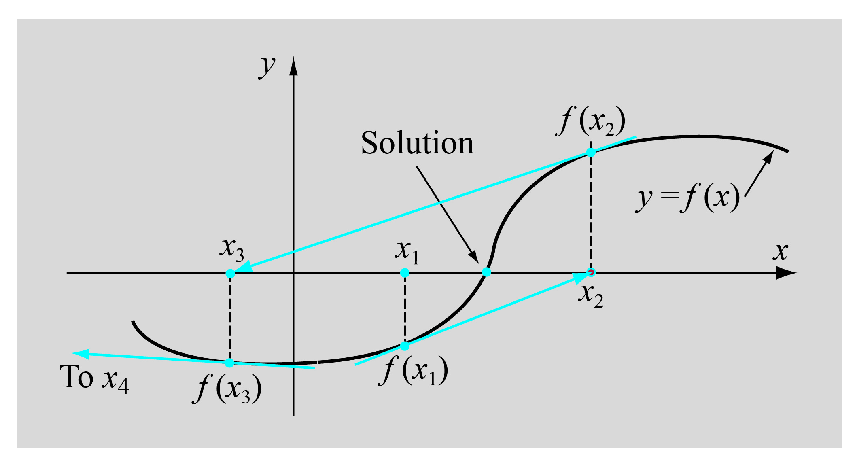
\includegraphics{Chapter3_Fig3_12a.eps}
\caption{Newton's method convergence issue due to a local minimum.}
\label{fig:lec4n-newton-troubles-a}
\end{marginfigure}

\item An inflection point can result in the iteration scheme entering into a cycle.  A schematic of this diabolical (and, thankfully, relatively uncommon) state of affairs is shown in Figure \ref{fig:lec4n-newton-troubles-b}.

\begin{marginfigure}
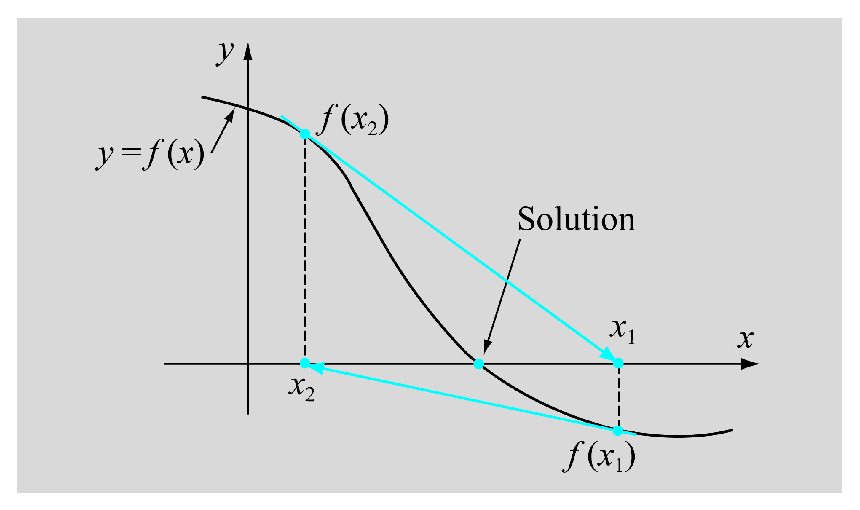
\includegraphics{Chapter3_Fig3_12b.eps}
\caption{Newton's method failure to converge due to inflection points in vicinity of solution.}
\label{fig:lec4n-newton-troubles-b}
\end{marginfigure}


\end{enumerate}
Notwithstanding these difficulties, it is possible to show that Newton's method will converge if the function, $f(x)$, and its first and second derivatives are all \emph{continuous}, and if the first derivitive is not zero at the solution, and if the starting value, $x_1$, is ``near'' the exact solution.\sidenote{Whatever the hell ``near'' is supposed to mean.}

